% (c) 2017 Daniele Zambelli - daniele.zambelli@gmail.com
% 
% Tutti i grafici per il capitolo relativo al piano cartesiano
%

\newcommand{\assea}{% Retta con numeri messi a caso.
    \disegno{
      \draw [-] (-6,0) -- (6,0) node [below]  {$x$};
      \foreach \x/\n in {-5/12, -2/0, 0/-7, 1/-3, 3.5/9, 5/5}
        \filldraw (\x, 0) circle (1.5pt) node [below] {\n};
    }
}

\newcommand{\asseb}{% Retta con numeri messi al posto giusto.
    \disegno{
      \draw [-] (-6,0) -- (6,0) node [below]  {$x$};
      \foreach \x in {-5, -3, -2, -1, 0, 1, 2, 3.5, 5}
        \filldraw (\x, 0) circle (1.5pt) node [below] {\x};
    }
}

\newcommand{\assec}{% Asse vuoto con l'indicazione dell'unità separata
    \disegnod{8}{
      \assex{-6}{6}{0}
      \draw[|-|] (0, .5) -- (1, .5) node[below, midway] {unità};
      \filldraw (0,0) circle (1.5pt) node [below] {0};
    }
}

\newcommand{\assed}{% Asse cartesiano con i trattini
    \disegnod{8}{
      \assecontrattini{-6}{6}{0}{\(x\)}
      \node [below] at (0, -.05) {0};
      \node [below] at (1, -.05) {1};
    }
}

% 
\newcommand{\assee}{% Asse cartesiano nei quadretti
    \disegnod{8}{
      \draw[step=1.0, gray!50, very thin] (-6.3, -1.2) grid (6.3, 1.2);
      \assex{-6.3}{6.3}{0}
      \draw [-] (0, -.05) -- (0, .1);
      \node [below] at (0,0) {0};
    }
}

\newcommand{\assef}{% Asse cartesiano con alcuni esempi di numeri
    \disegnod{8}{
      \assecontrattini{-6}{6}{0}{\(x\)}
%       \foreach \xi/\si in {-5, -4, ..., 1, 1.4142/\(\sqrt{2}\),
%                            2, 3, 3.5/\(\frac{7}{2}\), 4, 5, 
%                            -2.5/\(-\frac{5}{2}\)}
      \foreach \xi/\si in {-5, -4, -3, -1.5, 0, 1, 1.4,
                           2, 3, 3.5/\(\frac{7}{2}\), 6, 
                           -2.5/\(-\frac{5}{2}\)}
      \filldraw (\xi, 0)circle (1.5pt) node [below, yshift=-.1cm] {\si};
    }
}

\begin{comment}

%%%
% Asse cartesiano con alcuni esempi di punti
%%%%
\usepgflibrary{arrows.meta}

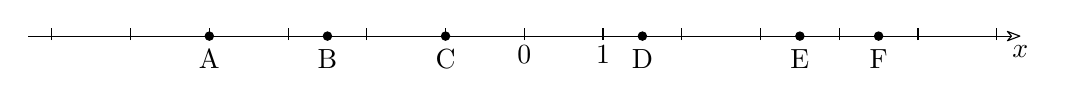
\begin{tikzpicture}[x=10mm, y=10mm, smooth]

%Asse cartesiano con trattini
% (c) 2014 Daniele Zambelli - daniele.zambelli@gmail.com

%%%
% Asse cartesiano con i trattini
%%%%
%Asse cartesiano con trattini
% \usepgflibrary{arrows.meta}

\draw [-{Stealth[length=2mm, open, round]}] (-6.3,0) -- (6.3,0) node [below]  {$x$};
\foreach \xi in {-6, -5, ..., 6}
\draw [-] (\xi, -.05) -- (\xi, .1);
\node [below] at (0, 0) {0};
\node [below] at (1, 0) {1};


\filldraw (-4, 0) circle (1.5pt) node [below, yshift=-.05cm] {A};
\filldraw (-2.5, 0) circle (1.5pt) node [below, yshift=-.05cm] {B};
\filldraw (-1, 0) circle (1.5pt) node [below, yshift=-.05cm] {C};
\filldraw (1.5, 0) circle (1.5pt) node [below, yshift=-.05cm] {D};
\filldraw (3.5, -0) circle (1.5pt) node [below, yshift=-.05cm] {E};
\filldraw (4.5, 0) circle (1.5pt) node [below, yshift=-.05cm] {F};

\end{tikzpicture}% (c) 2014 Daniele Zambelli - daniele.zambelli@gmail.com

%%%
% Asse cartesiano con alcuni esempi di punti
%%%%
\begin{tikzpicture}[x=5mm, y=5mm, smooth]

% (c) 2014 Daniele Zambelli - daniele.zambelli@gmail.com

%%%
% Asse cartesiano con i trattini
%%%%
%Asse cartesiano con trattini
% \usepgflibrary{arrows.meta}

\draw [-{Stealth[length=2mm, open, round]}] (-12.3, 0) -- (12.3, 0) node [below]  {$x$};
\foreach \xi in {-12, -11, ..., 12}
\draw [-] (\xi, -.05) -- (\xi, .1);
\node [below] at (0, 0) {0};
\node [below] at (1, 0) {1};


% Distanza tra punti entrambi di coordinata positiva
\filldraw (2, 0) circle (1.5pt) node [below, yshift=-.05cm] {A};
\filldraw (9, 0) circle (1.5pt) node [below, yshift=-.05cm] {B};

\end{tikzpicture}% (c) 2014 Daniele Zambelli - daniele.zambelli@gmail.com

%%%
% Asse cartesiano con alcuni esempi di punti
%%%%
\begin{tikzpicture}[x=5mm, y=5mm, smooth]

% (c) 2014 Daniele Zambelli - daniele.zambelli@gmail.com

%%%
% Asse cartesiano con i trattini
%%%%
%Asse cartesiano con trattini
% \usepgflibrary{arrows.meta}

\draw [-{Stealth[length=2mm, open, round]}] (-12.3, 0) -- (12.3, 0) node [below]  {$x$};
\foreach \xi in {-12, -11, ..., 12}
\draw [-] (\xi, -.05) -- (\xi, .1);
\node [below] at (0, 0) {0};
\node [below] at (1, 0) {1};


% Distanza tra punti entrambi di coordinata positiva
\filldraw (-8, 0) circle (1.5pt) node [below, yshift=-.05cm] {A};
\filldraw (-3, 0) circle (1.5pt) node [below, yshift=-.05cm] {B};

\end{tikzpicture}% (c) 2014 Daniele Zambelli - daniele.zambelli@gmail.com

%%%
% Asse cartesiano con alcuni esempi di punti
%%%%
\begin{tikzpicture}[x=5mm, y=5mm, smooth]

% (c) 2014 Daniele Zambelli - daniele.zambelli@gmail.com

%%%
% Asse cartesiano con i trattini
%%%%
%Asse cartesiano con trattini
% \usepgflibrary{arrows.meta}

\draw [-{Stealth[length=2mm, open, round]}] (-12.3, 0) -- (12.3, 0) node [below]  {$x$};
\foreach \xi in {-12, -11, ..., 12}
\draw [-] (\xi, -.05) -- (\xi, .1);
\node [below] at (0, 0) {0};
\node [below] at (1, 0) {1};


% Distanza tra punti entrambi di coordinata positiva
\filldraw (-5, 0) circle (1.5pt) node [below, yshift=-.05cm] {A};
\filldraw (7, 0) circle (1.5pt) node [below, yshift=-.05cm] {B};

\end{tikzpicture}% (c) 2014 Daniele Zambelli - daniele.zambelli@gmail.com

%%%
% Asse cartesiano con alcuni esempi di punti
%%%%
\begin{tikzpicture}[x=5mm, y=5mm, smooth]

% (c) 2014 Daniele Zambelli - daniele.zambelli@gmail.com

%%%
% Asse cartesiano con i trattini
%%%%
%Asse cartesiano con trattini
% \usepgflibrary{arrows.meta}

\draw [-{Stealth[length=2mm, open, round]}] (-12.3, 0) -- (12.3, 0) node [below]  {$x$};
\foreach \xi in {-12, -11, ..., 12}
\draw [-] (\xi, -.05) -- (\xi, .1);
\node [below] at (0, 0) {0};
\node [below] at (1, 0) {1};


% Distanza tra punti entrambi di coordinata positiva
\filldraw (7, 0) circle (1.5pt) node [below, yshift=-.05cm] {A};
\filldraw (2, 0) circle (1.5pt) node [below, yshift=-.05cm] {B};

\end{tikzpicture}% (c) 2014 Daniele Zambelli - daniele.zambelli@gmail.com

%%%
% Asse cartesiano con alcuni esempi di punti
%%%%
\begin{tikzpicture}[x=5mm, y=5mm, smooth]

% (c) 2014 Daniele Zambelli - daniele.zambelli@gmail.com

%%%
% Asse cartesiano con i trattini
%%%%
%Asse cartesiano con trattini
% \usepgflibrary{arrows.meta}

\draw [-{Stealth[length=2mm, open, round]}] (-12.3, 0) -- (12.3, 0) node [below]  {$x$};
\foreach \xi in {-12, -11, ..., 12}
\draw [-] (\xi, -.05) -- (\xi, .1);
\node [below] at (0, 0) {0};
\node [below] at (1, 0) {1};


% Distanza tra punti entrambi di coordinata positiva
\filldraw (3, 0) circle (1.5pt) node [below, yshift=-.05cm] {A};
\filldraw (9, 0) circle (1.5pt) node [below, yshift=-.05cm] {B};

\end{tikzpicture}% (c) 2014 Daniele Zambelli - daniele.zambelli@gmail.com

\end{comment}

\newcommand{\assistrani}{% Assi non ortogonali monometrici
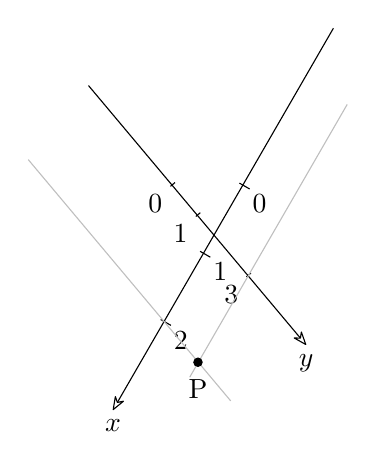
\begin{tikzpicture}[smooth]
  \begin{scope}[x=10mm, y=10mm, xshift=9mm, rotate=-120]
  \draw [-{Stealth[length=2mm, open, round]}] (-2.3, 0) -- (3.3, 0) node 
  [below] {$x$};
  \draw [-] (0, -.05) -- (0, .1) node [below right] at (0, 0) {0};
  \draw [-] (1, -.05) -- (1, .1) node [below right] at (1, 0) {1};
  \draw [-] (2, -.05) -- (2, .1) node [below right] at (2, 0) {2};
  \draw [-] [gray!50, rotate=-20](1.88, -2) -- (1.88, 2);
  \end{scope}

  \begin{scope}[x=5mm, y=5mm, rotate=-50]
  \draw [-{Stealth[length=2mm, open, round]}] (-3.3, 0) -- (5.3, 0) node 
  [below] {$y$};
  \draw [-] (0, -.05) -- (0, .1) node [below left] at (0, 0) {0};
  \draw [-] (1, -.05) -- (1, .1) node [below left] at (1, 0) {1};
  \draw [-] (3, -.05) -- (3, .1) node [below left] at (3, 0) {3};
  \draw [-] [gray!50, rotate=20](2.83, -4) -- (2.83, 4);
  \end{scope}

  \filldraw (0.33, -2.25) circle (1.5pt) node [below, yshift=-.1cm] {P};
\end{tikzpicture}
}

\newcommand{\assinormali}{% Piano cartesiano ortogonale monometrico
    \disegno{
      \rcom{-5}{+5}{-5}{+5}{gray!50, very thin, step=1}
      \filldraw (2, 3) circle (1.5pt) node [below, yshift=-.1cm] {P};
    }
}

\newcommand{\pianoconquadranti}{% Piano cartesiano con indicati i quadranti
    \disegno{
      \rcom{-5}{+5}{-5}{+5}{gray!50, very thin, step=1}
      \node at (2.5, 2.5) {I quadrante};
      \node at (-2.5, 2.5) {II quadrante};
      \node at (-2.5, -2.5) {III quadrante};
      \node at (2.5, -2.5) {IV quadrante};
    }
}

\newcommand{\pianoconsegni}{% Piano cartesiano con segni delle coordinate
    \disegno{
      \rcom{-5}{+5}{-5}{+5}{gray!50, very thin, step=1}
      \node at (2.5, 2.5) {$(+; +)$};
      \node at (-2.5, 2.5) {$(-; +)$};
      \node at (-2.5, -2.5) {$(-; -)$};
      \node at (2.5, -2.5) {$(+; -)$};
    }
}

\newcommand{\puntineiqadr}{% Piano cartesiano punti nei quadranti
    \disegno{
      \rcom{-5}{+5}{-5}{+5}{gray!50, very thin, step=1}
      \foreach \pos/\lab in {(2, 3)/A, (-1, 4)/B, (-3, -2)/C, (4, -3)/D}
        \filldraw \pos circle (1.5pt) node [below, xshift=5pt] {\lab};
    }
}

\newcommand{\puntisugliassi}{% Piano cartesiano punti sugli assi
    \disegno{
      \rcom{-5}{+5}{-5}{+5}{gray!50, very thin, step=1}
      \foreach \pos/\lab in {(0, 4)/R, (0, -2)/S, (-4, 0)/H, (3, 0)/K}
        \filldraw \pos circle (1.5pt) node [below, xshift=5pt] {\lab};
    }
}

\newcommand{\puntomedio}{% Punto medio di un segmento
    \disegno{
      \rcom{-3}{+10}{-2}{+8}{gray!50, very thin, step=1}
      \coordinate (a) at (2, 3);
      \coordinate (b) at (8, 6);
      \coordinate (m) at ($ (a)!.5!(b) $);
      \draw [-] (a) -- (b);
      \filldraw (a) circle (1.5pt) node [below right] {A};
      \filldraw (b) circle (1.5pt) node [below right] {B};

      \begin{scope}[dotted]
      \draw [-] (a) -- (2, 0) node [below] {$x_A$};
      \draw [-] (a) -- (0, 3) node [left] {$y_A$};
      \draw [-] (b) -- (8, 0) node [below] {$x_B$};
      \draw [-] (b) -- (0, 6) node [left] {$y_B$};
      \begin{scope}[red]
      \filldraw (m) circle (1.5pt) node [below right] {M};
      \draw [-] (m) -- (5, 0) 
        node [below, xshift=2pt] {$\dfrac{x_{A}+x_{B}}{2}$};
      \draw [-] (m) -- (0, 4.5) 
        node [left, yshift=2pt] {$\dfrac{y_{A}+y_{B}}{2}$};
      \end{scope}
      \end{scope}
    }
}

\newcommand{\segmentiparalleli}{% Segmenti parallelia agli assi
    \disegno{
      \rcom{-5}{+5}{-5}{+5}{gray!50, very thin, step=1}
      \coordinate (a) at (-2, 3);
      \coordinate (b) at (4, 3);
      \draw [-] (a) -- (b);
      \filldraw (a) circle (1.5pt) node [below right] {A};
      \filldraw (b) circle (1.5pt) node [below right] {B};

      \begin{scope}[dotted]
      \draw [-] (a) -- (-2, 0) node [below] {$x_A$};
      \draw [-] (b) -- (4, 0) node [below] {$x_B$};
      \end{scope}

      \coordinate (c) at (-4, -3);
      \coordinate (d) at (-4, 2);
      \draw [-] (c) -- (d);
      \filldraw (c) circle (1.5pt) node [below right] {C};
      \filldraw (d) circle (1.5pt) node [below right] {D};

      \begin{scope}[dotted]
      \draw [-] (c) -- (0, -3) node [right] {$y_C$};
      \draw [-] (d) -- (0, 2) node [right] {$y_D$};
      \end{scope}
    }
}

\newcommand{\lungseg}{% Segmento qualunque
    \disegno{
      \rcom{-5}{+5}{-5}{+5}{gray!50, very thin, step=1}
      \foreach \pos/\lab in {(0, 4)/R, (0, -2)/S, (-4, 0)/H, (3, 0)/K}
      \coordinate (e) at (-3, -4);
      \coordinate (f) at (2, 4);
      \coordinate (g) at (2, -4);
      \draw [-] (e) -- (f);
      \filldraw (e) circle (1.5pt) node [below right] {E};
      \filldraw (f) circle (1.5pt) node [below right] {F};
      \filldraw (g) circle (1.5pt) node [below right] {G};

      \begin{scope}[dotted]
      \draw [-] (e) -- (g) 
        node [below, xshift=1mm] at ($(e)!.5!(g)$) {$x_F - x_E$};
      \draw [-] (f) -- (g) 
        node [below, xshift=8mm] at ($(f)!.5!(g)$) {$y_F - y_E$};
      \end{scope}
    }
}

\newcommand{\areasottesauno}{% Area sottesa a un segmento
    \disegno{
      \coordinate (a) at (1, 3);
      \coordinate (xa) at (1, 0);
      \coordinate (ya) at (0, 3);
      \coordinate (b) at (7, 8);
      \coordinate (xb) at (7, 0);
      \coordinate (yb) at (0, 8);

      \fill [top color=green!30!black!20,bottom color=green!50!black!10] 
      (a) -- (b) -- (xb) -- (xa) -- cycle;

      \rcom{-1}{+9}{-1}{+9}{gray!50, very thin, step=1}
      
      \draw [-] (a) -- (b);
      \filldraw (a) circle (1.5pt) node [below right] {A};
      \filldraw (b) circle (1.5pt) node [below right] {B};

      \begin{scope}[dotted]
      \draw [-] (a) -- (xa) node [below] {$A'$};
      \draw [-] (a) -- (ya) node [left] {$y_A$};
      \draw [-] (b) -- (xb) node [below] {$B'$};
      \draw [-] (b) -- (yb) node [left] {$y_B$};
      \end{scope}
    }
}

\newcommand{\areasottesamolti}{% Area sottesa a più segmenti
    \disegno{
      \coordinate (a) at (-7, 3);
      \coordinate (xa) at (-7, 0);
      \coordinate (b) at (-4, 8);
      \coordinate (xb) at (-4, 0);
      \coordinate (c) at (2, 8);
      \coordinate (xc) at (2, 0);
      \coordinate (d) at (6, 0);
      \coordinate (xd) at (6, 0);

      \fill [top color=green!40!black!20,bottom color=green!80!black!05] 
      (a) -- (b) -- (xb) -- (xa) -- cycle;
      \fill [top color=orange!80!black!05,bottom color=orange!40!black!20] 
      (b) -- (c) -- (xc) -- (xb) -- cycle;
      \fill [top color=purple!40!black!20,bottom color=purple!80!black!05] 
      (c) -- (d) -- (xd) -- (xc) -- cycle;
        
      \rcom{-9}{+9}{-1}{+9}{gray!50, very thin, step=1}

      \draw [-] (a) -- (b) --(c) --(d);
      \filldraw (a) circle (1.5pt) node [above] {A};
      \filldraw (b) circle (1.5pt) node [above] {B};
      \filldraw (c) circle (1.5pt) node [above] {C};
      \filldraw (d) circle (1.5pt) node [above] {D};

      \begin{scope}[dotted]
      \draw [-] (a) -- (xa) node [below] {$A'$};
      \draw [-] (b) -- (xb) node [below] {$B'$};
      \draw [-] (c) -- (xc) node [below] {$C'$};
      \draw [-] (d) -- (xd) node [below] {$D'$};
      \end{scope}
    }
}

\newcommand{\triangoloerone}{% Area triangolo con la formula di Erone
    \disegno{
      \coordinate (a) at (-4, -3);
      \coordinate (b) at (3, -1);
      \coordinate (c) at (2, 4);

      \fill [top color=green!30!black!20,bottom color=green!50!black!10] 
      (a) -- (b) -- (c) -- cycle;

      \rcom{-5}{+5}{-5}{+5}{gray!50, very thin, step=1}

      \draw [-] (a) -- (b) --(c) -- cycle;
      \filldraw (a) circle (1.5pt) node [below left] {A};
      \filldraw (b) circle (1.5pt) node [below right] {B};
      \filldraw (c) circle (1.5pt) node [above right] {C};
    }
}

\newcommand{\triangolodifferenza}{% Area triangolo ottenuto per differenza
    \disegno{
      \coordinate (a) at (-4, -3);
      \coordinate (b) at (3, -1);
      \coordinate (c) at (2, 4);
      \coordinate (d) at (3, -3);
      \coordinate (e) at (3, 4);
      \coordinate (f) at (-4, 4);

      \fill [top color=green!80!black!05,bottom color=green!40!black!20] 
      (a) -- (d) -- (e) -- (f) -- cycle;

      \fill [top color=red!40!black!20,bottom color=red!80!black!05] 
      (a) -- (b) -- (c) -- cycle;

      \rcom{-5}{+5}{-5}{+5}{gray!50, very thin, step=1}

      \draw [-] (a) -- (b) --(c) -- cycle;
      \filldraw (a) circle (1.5pt) node [below left] {A};
      \filldraw (b) circle (1.5pt) node [below right] {B};
      \filldraw (c) circle (1.5pt) node [above right] {C};
      \filldraw (d) circle (1.5pt) node [below left] {D};
      \filldraw (e) circle (1.5pt) node [below right] {E};
      \filldraw (f) circle (1.5pt) node [above right] {F};
    }
}

\newcommand{\triangoloparallelox}{% Triangolo con lato parallelo asse x
    \disegno{
      \coordinate (a) at (-4, 4);
      \coordinate (b) at (3, 4);
      \coordinate (c) at (2, -3);

      \fill [top color=green!30!black!20,bottom color=green!50!black!10] 
      (a) -- (b) -- (c) -- cycle;

      \rcom{-5}{+5}{-5}{+5}{gray!50, very thin, step=1}

      \draw [-] (a) -- (b) --(c) -- cycle;
      \filldraw (a) circle (1.5pt) node [below left] {A};
      \filldraw (b) circle (1.5pt) node [below right] {B};
      \filldraw (c) circle (1.5pt) node [above right] {C};
    }
}

\newcommand{\triangoloparalleloy}{% Triangolo con lato parallelo asse y
    \disegno{
      \coordinate (a) at (-4, 4);
      \coordinate (b) at (-4, 1);
      \coordinate (c) at (3, -4);

      \fill [top color=red!30!black!20,bottom color=red!50!black!10] 
      (a) -- (b) -- (c) -- cycle;

      \rcom{-5}{+5}{-5}{+5}{gray!50, very thin, step=1}

      \draw [-] (a) -- (b) --(c) -- cycle;
      \filldraw (a) circle (1.5pt) node [below left] {A};
      \filldraw (b) circle (1.5pt) node [below right] {B};
      \filldraw (c) circle (1.5pt) node [above right] {C};
    }
}
